% LaTeX template for academic reports (thesis)

\documentclass[12pt,english,a4paper,oneside]{article}
\let\circledS\undefined
\usepackage{setspace}
\setstretch{2.0}
\usepackage{amssymb,amsmath}
\usepackage{ifxetex,ifluatex}
\usepackage[nottoc]{tocbibind}
\usepackage{csquotes}
\usepackage[usenames,dvipsnames]{xcolor}
\usepackage[bookmarks, colorlinks, breaklinks]{hyperref}
\definecolor{mannheimblue}{HTML}{003056}
\definecolor{mannheimorange}{HTML}{df7e50}

\hypersetup{linkcolor=mannheimblue,
citecolor=mannheimblue,
filecolor=black,
urlcolor=mannheimblue}


% some more packages...
\usepackage{graphicx}
%\usepackage{scrpage2}
%\usepackage{xcolor}
\usepackage{hyperref}
%\hypersetup{colorlinks=true, linkcolor = blue, urlcolor = blue}
%\usepackage{eso-pic}

\renewenvironment{quote}{\list{}\item\relax
\small\singlespacing}{\endlist}
\SetBlockEnvironment{quote}

\onehalfspacing
% \renewcommand{\baselinestretch}{1.5}  % line distance is 1.5

%\renewcommand{\chaptername}{} %% remove the word \chapter

% % \newlength{\cslhangindent}
% \setlength{\cslhangindent}{1.5em}
% \newenvironment{CSLReferences}%
%   {\setlength{\parindent}{0pt}%
%   \everypar{\setlength{\hangindent}{\cslhangindent}}\ignorespaces}%
%   {\par}
% 
% Pandoc citation processing
\newlength{\cslhangindent}
\setlength{\cslhangindent}{1.5em}
\newlength{\csllabelwidth}
\setlength{\csllabelwidth}{3em}
\newlength{\cslentryspacingunit} % times entry-spacing
\setlength{\cslentryspacingunit}{\parskip}
% for Pandoc 2.8 to 2.10.1
\newenvironment{cslreferences}%
  {\setlength{\parindent}{0pt}%
  \everypar{\setlength{\hangindent}{\cslhangindent}}\ignorespaces}%
  {\par}
% For Pandoc 2.11+
\newenvironment{CSLReferences}[2] % #1 hanging-ident, #2 entry spacing
 {% don't indent paragraphs
  \setlength{\parindent}{0pt}
  % turn on hanging indent if param 1 is 1
  \ifodd #1
  \let\oldpar\par
  \def\par{\hangindent=\cslhangindent\oldpar}
  \fi
  % set entry spacing
  \setlength{\parskip}{#2\cslentryspacingunit}
 }%
 {}
\usepackage{calc}
\newcommand{\CSLBlock}[1]{#1\hfill\break}
\newcommand{\CSLLeftMargin}[1]{\parbox[t]{\csllabelwidth}{#1}}
\newcommand{\CSLRightInline}[1]{\parbox[t]{\linewidth - \csllabelwidth}{#1}\break}
\newcommand{\CSLIndent}[1]{\hspace{\cslhangindent}#1}
% % \newlength{\cslhangindent}
% \setlength{\cslhangindent}{1.5em}
% \newlength{\csllabelwidth}
% \setlength{\csllabelwidth}{3em}
% \newenvironment{CSLReferences}[3] % #1 hanging-ident, #2 entry spacing
%  {% don't indent paragraphs
%   \setlength{\parindent}{0pt}
%   % turn on hanging indent if param 1 is 1
%   \ifodd #1 \everypar{\setlength{\hangindent}{\cslhangindent}}\ignorespaces\fi
%   % set entry spacing
%   \ifnum #2 > 0
%   \setlength{\parskip}{#2\baselineskip}
%   \fi
%  }%
%  {}
% \usepackage{calc} % for \widthof, \maxof
% \newcommand{\CSLBlock}[1]{#1\hfill\break}
% \newcommand{\CSLLeftMargin}[1]{\parbox[t]{\maxof{\widthof{#1}}{\csllabelwidth}}{#1}}
% \newcommand{\CSLRightInline}[1]{\parbox[t]{\linewidth}{#1}}
% \newcommand{\CSLIndent}[1]{\hspace{\cslhangindent}#1}
% 
\usepackage{fixltx2e} % provides \textsubscript
\ifnum 0\ifxetex 1\fi\ifluatex 1\fi=0 % if pdftex
  \usepackage[T1]{fontenc}
  \usepackage[utf8]{inputenc}
\else % if luatex or xelatex
  \ifxetex
    \usepackage{mathspec}
  \else
    \usepackage{fontspec}
  \fi
  \defaultfontfeatures{Ligatures=TeX,Scale=MatchLowercase}

\fi
% % use upquote if available, for straight quotes in verbatim environments
% \IfFileExists{upquote.sty}{\usepackage{upquote}}{}
% % use microtype if available
% \IfFileExists{microtype.sty}{%
% \usepackage{microtype}
% \UseMicrotypeSet[protrusion]{basicmath} % disable protrusion for tt fonts
% }{}
% % \usepackage[left=2.5cm,right=2.5cm,top=2.5cm,bottom=2.5cm]{geometry}
% \usepackage{hyperref}
\hypersetup{unicode=true,
            pdftitle={Evaluating UN peace-keeping Operations},
            pdfauthor={Tobias Stenzel},
            pdfborder={0 0 0},
            breaklinks=true}
\urlstyle{same}  % don't use monospace font for urls
\ifnum 0\ifxetex 1\fi\ifluatex 1\fi=0 % if pdftex
  \usepackage[shorthands=off,main=english]{babel}
\else
  \usepackage{polyglossia}
  \setmainlanguage[]{english}
\fi
% % \usepackage{longtable,booktabs}
\setlength{\emergencystretch}{3em}  % prevent overfull lines
\providecommand{\tightlist}{%
  \setlength{\itemsep}{0pt}\setlength{\parskip}{0pt}}
\setcounter{secnumdepth}{5}
% Redefines (sub)paragraphs to behave more like sections
\ifx\paragraph\undefined\else
\let\oldparagraph\paragraph
\renewcommand{\paragraph}[1]{\oldparagraph{#1}\mbox{}}
\fi
\ifx\subparagraph\undefined\else
\let\oldsubparagraph\subparagraph
\renewcommand{\subparagraph}[1]{\oldsubparagraph{#1}\mbox{}}
\fi


\usepackage{csquotes}
\usepackage{fancyhdr} % to change header and footers
\usepackage{url}
\def\UrlBreaks{\do\/\do-}

%%%% plagiarism

\newcommand*{\SignatureAndDate}[1]{%
\vspace{2cm}
     Mannheim, den \makebox[2cm]{\hrulefill} \hfill\makebox[9cm]{\hrulefill}%
     \par
%  \makebox[2cm]{ Ort, Datum}
  \hfill\makebox[7.5cm][t]{Name und Unterschrift}
  \vspace{2cm}
}%

 \newcommand*{\SignatureAndDateEng}[1]{%
\vspace{2cm}
     Mannheim, \makebox[2cm]{\hrulefill} \hfill\makebox[9cm]{\hrulefill}%
     \par
    \hfill\makebox[7.5cm][t]{Name and Signature}%
\vspace{2cm}
}%


\makeatletter
\newenvironment{kframe}{%
\medskip{}
\setlength{\fboxsep}{.8em}
 \def\at@end@of@kframe{}%
 \ifinner\ifhmode%
  \def\at@end@of@kframe{\end{minipage}}%
  \begin{minipage}{\columnwidth}%
 \fi\fi%
 \def\FrameCommand##1{\hskip\@totalleftmargin \hskip-\fboxsep
 \colorbox{shadecolor}{##1}\hskip-\fboxsep
     % There is no \\@totalrightmargin, so:
     \hskip-\linewidth \hskip-\@totalleftmargin \hskip\columnwidth}%
 \MakeFramed {\advance\hsize-\width
   \@totalleftmargin\z@ \linewidth\hsize
   \@setminipage}}%
 {\par\unskip\endMakeFramed%
 \at@end@of@kframe}
\makeatother

%\renewenvironment{Shaded}{\begin{kframe}}{\end{kframe}} ses 2019-03-08












\newcommand{\ts}{\thinspace}



\usepackage{tikz, float, caption}
\floatplacement{figure}{H}
\interfootnotelinepenalty=10000

%% font EB Garamond
\setmainfont[
Path = fonts/static/,
BoldFont = EBGaramond-Bold.ttf,
ItalicFont = EBGaramond-Italic.ttf,
BoldItalicFont  = EBGaramond-BoldItalic.ttf]
{EBGaramond-Regular.ttf}


% \usepackage{float}

\begin{document}  %%%%%%% main document %%%%%%%%%%%%%%%
\begin{titlepage}

    \begin{center}
    \large{ \textsc{ \uppercase{University of Mannheim} \\ \vspace{-0.2cm}
School of Social Sciences \\ \vspace{-0.2cm}
Department of Political Science}}

      
        \vspace{3.5cm}
        

       \large{   Data Essay for Course   }


       \large{ \textit{   Quantitative Methods in Political Science   }}

\renewcommand{\linethickness}{0.03em}
\rule{\linewidth}{\linethickness}


       \LARGE{ \textbf{   Evaluating UN peace-keeping Operations   }}

        % \vspace{-0.5cm}

       \large{  }

        \vspace{-0.2cm}
\rule{\linewidth}{\linethickness}


\begin{minipage}[t]{0.5\textwidth}
\begin{flushleft}
\singlespacing
 \textbf{Tobias Stenzel}  \\ 


 \href{mailto:tobias.stenzel@students.uni-mannheim.de}{\nolinkurl{tobias.stenzel@students.uni-mannheim.de}}  \\ 

\end{flushleft}
\end{minipage}
\begin{minipage}[t]{0.4\textwidth}
\hfill
\end{minipage}\\
\vspace{0.2cm}
\begin{minipage}[t]{0.35\textwidth}
\hfill
\end{minipage}
\begin{minipage}[t]{0.55\textwidth}
\begin{flushright}
\singlespacing
     Prof.~Thomas Gschwend, Ph.D.  \\       

\end{flushright}
\end{minipage}\\
%


         \vfill
         Submission Date: Dezember 15, 2021 \\ 
        





         \vfill



     \end{center}
    \thispagestyle{empty}
\end{titlepage}

\newpage
% \thispagestyle{empty}
% \mbox{}







{
\setcounter{tocdepth}{2}
\newpage
\pagenumbering{gobble}
\tableofcontents
}

\newpage
\pagenumbering{arabic}
\fancypagestyle{plain}{%
    \renewcommand{\headrulewidth}{0pt}%
    \fancyhf{}%
    \fancyfoot[R]{\thepage}%
}
% Set the right side of the footer to be the page number
\pagestyle{plain}
\hypertarget{empirical-strategy}{%
\section{Empirical Strategy}\label{empirical-strategy}}

\hypertarget{selection-of-variables}{%
\subsection{Selection of variables}\label{selection-of-variables}}

We analyze two hypotheses in this essay. The first hypothesis (H1) is that an increased number of UN troops tends to decrease fatalities of inner-state conflicts. The second hypothesis (H2) is that this effect tends to be more pronounced when conflict parties are willed to settle the conflict.

To test both hypotheses, we need to analyze the interplay of the number of UN peace-keeping troops and the actors' willingness for conflict resolution and its effect on battle-related fatalities. I illustrate the relationships between those variables in Figure 1: \emph{willingness} (M) moderates the effect of \emph{UN forces} (X) on \emph{fatalities} (Y). Furthermore, we have to account for four variables (C) that potentially confound the relationship between our two main independent variables and the outcome variable.

The first one of these confounders is \emph{rebel strength}. Arguably, a more powerful rebel opposition requires a higher number of UN troops as it has a larger potential to cause fatalities. The second confounder is \emph{number of rebel groups}. A larger number of rebel groups may weaken the opposition due to higher coordination costs. Thus, its effect would have the opposite direction of rebel strength. The third and fourth confounders are whether a \emph{regional} peace-keeping operation (\emph{PKO}) or a state supports the UN mission. Conceivably, both variables reduce the number of required UN troops. However, regional PKO may reduce the number of fatalities, whereas \emph{state intervention} may increase this number because the respective states may have a hidden agenda.

\begin{figure}[H]
\label{fig:causal}
\centering

  \begin{tikzpicture}[node distance={25mm}, thick, main/.style = {draw, circle}]
  
  
    \node[main] (M) {$M$}; 
    \node[main] (C) [right of=M] {$C$};
    \node[main] (Y) [below of=C] {$Y$};     
    \node[main] (X) [below of=M] {$X$}; 
  
    \draw[->] (X) -- (M); 
    \draw[->] (X) -- (Y);
    
    \draw[->] (C) -- (X);
    \draw[->] (C) -- (Y);
    \draw[->] (C) -- (M);
    
    \draw[->] (M) -- (Y); 
  \end{tikzpicture}
  
  \caption{Causal relationship between the number of UN peace-keeping forces, actors' willingness to resolve the conflict and battle-related fatalities}

\end{figure}

\hypertarget{data}{%
\subsection{Data}\label{data}}

The dataset contains 3345 monthly observations from 38 active conflicts between 1990 and 2011. The number of UN forces includes both military and police. Fatalities are measured monthly and include civilians and armed forces. Fatalities should be measured relative to the population size. Therefore, we will consider the monthly fatality rate per Mio. inhabitants. Rebel strength is measured in proportion to the government on a scale from one to five. Three represents a level similar to the government. Willingness is measured by whether a ceasefire agreement exists or not. State intervention and regional PKO are binary variables as well.

\hypertarget{methodology}{%
\subsection{Methodology}\label{methodology}}

Since the number of fatalities is an overdispersed count variable, I use negative binomial models. Furthermore, I include population as an offset variable for two reasons: First, as mentioned above, I want to consider the monthly rate of fatalities per population. Second, as pointed out by Agresti (2015)\footnote{See page 233.}, using the ratio directly as an independent variable results in biased standard errors. Therefore, it is better to use the denominator variable as an offset. I test several models that gradually include (1) simple additive effects of UN forces and ceasefire, (2) their interaction, and (3) their interaction adjusting for potential confounders. For better comparability of the models, I restrict the data to observations for which the complete set of variables is available. According to hypotheses H1 and H2, we would expect positive effects for UN troops and its interaction with a ceasefire on the fatality rate.

\phantom{This text will be invisible}

\noindent
To illustrate my findings, I simulate expected values for the independent variable fatalities for different scenarios. In this study, I also analyze the interplay between the two main independent variables over the full range of UN troops to inspect the shape of this relation.\footnote{Note that expected values underestimate the total uncertainty because they do only include the estimation uncertainty but not the fundamental uncertainty.}

\hypertarget{descriptive-statistics}{%
\section{Descriptive Statistics}\label{descriptive-statistics}}

In this section, we take a closer look at the distributions of our variables. This will help us distinguish typical and unusual values or events and improve our intuition about their relations. Moreover, we can use our insights to select interesting scenarios for analyzing the substantial effects of our main variables.

\phantom{This text will be invisible}

\begin{figure}[H]
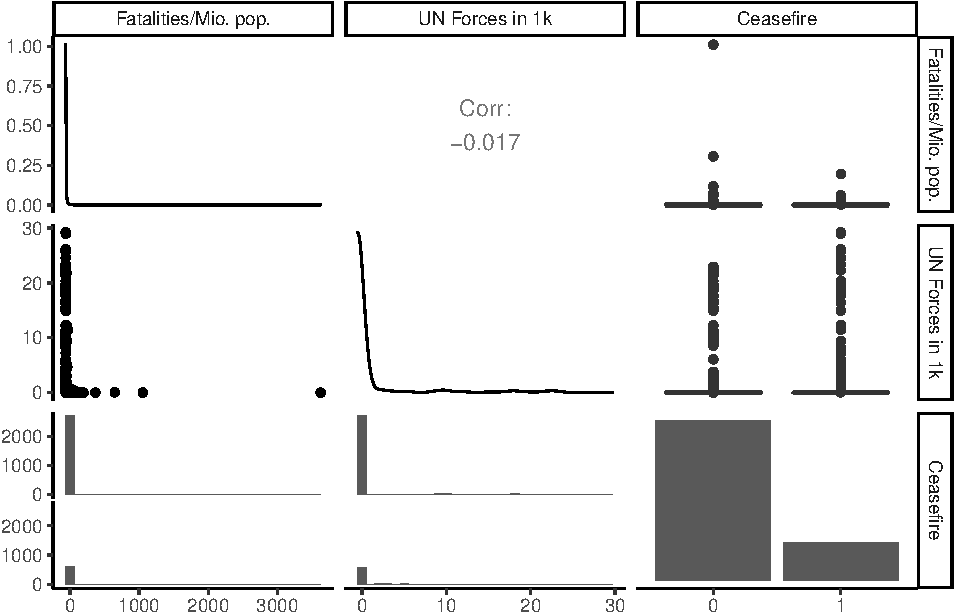
\includegraphics[width=\textwidth]{figs/desc-main-1} \caption[Distribution and relationships of main variables]{Distribution and relationships of main variables.}\label{fig:desc-main}
\vspace{0.5cm} \footnotesize{\textit{Notes: }Fatalities/Mio. pop. are monthly.} \end{figure}

\noindent
Figure \ref{fig:desc-main} shows the distributions of our main variables. The first column depicts the monthly rate of fatalities per million inhabitants. It has mean 5.2 and standard deviation 67. We see that it approximately follows the power law. This means that most of the values are very low, i.e., close to 0, but the distribution has a long tail. Accurately modeling the latter property is challenging because most distribution cannot account for non-zero probabilities for very extreme events. We also observe an extreme outlier: In June 1997, 9793 people were killed in the conflict between the state of Congo and the rebel group Cobras. As extreme values are arguably a defining property of this DGP, such outliers should not be removed. The second row shows that the most extreme fatality rates did not occur in the presence of substantial UN forces.

\noindent
The second column depicts the distribution of UN forces. Its mean and standard deviation are 1.1 and 4.0, respectively. This count distribution has a similar shape to the previous with less pronounced extremes. The highest number of UN forces was counted in 1993 in Somalia as 29,209. This variable is almost uncorrelated with fatalities.
The third column shows the binary distribution of ceasefire. We see a ceasefire agreement in 19\% of the observations. However, if there is an agreement, UN forces tend to be larger.

\noindent
Figure \ref{fig:desc-conf} presents the distributions of our controls. Light gray depicts the contributions from observations with a ceasefire and dark grey without a ceasefire. We observe that rebel groups, in most cases, are weaker than the government. However, with increasing strength, the frequency of ceasefire agreements also increases. The same two trends are also true for the number of rebel groups. In some cases, the number is surprisingly high. Finally, the distribution of state intervention and regional PKO is almost identical. The two events have a frequency of 16\% and 17\%, respectively. However, the correlation between both variables is only about 7\%. Therefore, it appears as if their roles are somewhat similar and that both events tend to substitute each other.

\phantom{This text will be invisible}

\begin{figure}[H]
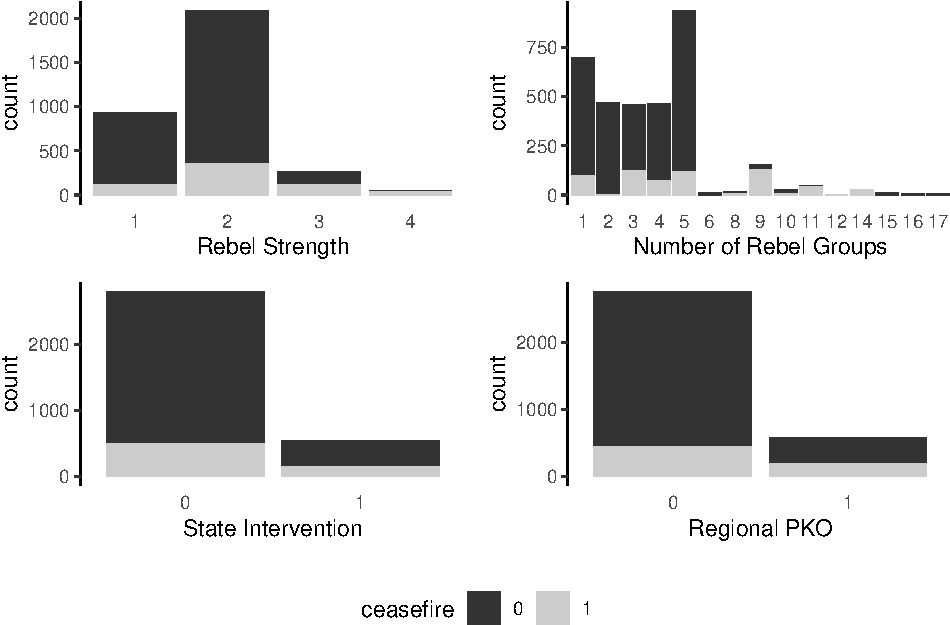
\includegraphics[width=\textwidth]{figs/desc-conf-1} \caption[Distribution of potential confounders]{Distribution of potential confounders.}\label{fig:desc-conf}
\end{figure}

\hypertarget{results}{%
\section{Results}\label{results}}

\hypertarget{regression-results}{%
\subsection{Regression Results}\label{regression-results}}

Table \ref{tab:table} shows the results of the negative binomial regression analyses for H1 and H2. Model (1) shows purely additive effects. For a typical observation with reference-level variable values, the intercept equals the log fatality rate, i.e., the number of monthly fatalities per Mio. inhabitants. The coefficients show how much a one-unit increase in the respective covariate increases the log of the fatality rate. This results in the following interpretations: In model (1), the reference fatality rate is 4.92. If a thousand UN forces were deployed, the rate would have decreased by 11.\% (or the log would have decreased by 0.122). This finding agrees with H1. However, if the parties had agreed to a ceasefire, the rate would have increased by 157\%. Model (2) adds the interaction effect between both dependent variables. It has the following interpretation: If there is a ceasefire, an increase in UN forces by 1k results in an increase of monthly fatalities per mio inhabitants by 102\%. This result contradicts H2. Model (3), however, tests whether these findings are robust to the four confounders. We can see that the direction of the interaction effect changes from model (2) to model (3) into the direction suggested by H2. The effects of UN forces, ceasefire and their interaction on fatalities are now -17\%, +132\%, and -8\%, respectively. Moreover, the effects of our controls rebel strength, number of rebel groups, state intervention, and regional PKO are +214\%, -4\%, +271\%, and -45\%. We interpret variables separately, holding all others constant at their reference values. According to all measures of goodness of fit, the best model is model (3). There, all coefficients except the number of rebel groups are highly significant.

\hypertarget{model-fit}{%
\subsection{Model Fit}\label{model-fit}}

As mentioned in the methodology section, I use the likelihood ratio test to decide whether I can use the simpler Poisson model instead. Nevertheless, the tests suggest the negative binomial model for all models due to overdispersion. However, to decide which specific model specification is best, I consider the Akaike information criterion (AIC). The intuition is that a higher model likelihood can also be solely because more covariates are included. Therefore, the AIC penalizes the number of model variables. Unsurprisingly, model (3) has the best fit according to the AIC. Another interesting fact is that model (2) with the interaction term is worse than baseline model (1).

\begin{table}[!htbp] \centering 
  \caption{Regression Results} 
  \label{tab:table} 
\begin{tabular}{@{\extracolsep{5pt}}lccc} 
\\[-1.8ex]\hline 
\hline \\[-1.8ex] 
 & \multicolumn{3}{c}{\textit{Dependent variable:}} \\ 
\cline{2-4} 
\\[-1.8ex] & \multicolumn{3}{c}{Monthly fatalities / pop. in Mio.} \\ 
\\[-1.8ex] & (1) & (2) & (3)\\ 
\hline \\[-1.8ex] 
 UN Forces in 1k & $-$0.122$^{***}$ & $-$0.128$^{***}$ & $-$0.075$^{***}$ \\ 
  & (0.014) & (0.016) & (0.017) \\ 
  & & & \\ 
 Ceasefire & 0.461$^{***}$ & 0.427$^{***}$ & 0.843$^{***}$ \\ 
  & (0.145) & (0.152) & (0.162) \\ 
  & & & \\ 
 Rebel Strength &  &  & 1.143$^{***}$ \\ 
  &  &  & (0.098) \\ 
  & & & \\ 
 Number Rebel Groups &  &  & $-$0.039$^{*}$ \\ 
  &  &  & (0.022) \\ 
  & & & \\ 
 Biased Intervention &  &  & 1.310$^{***}$ \\ 
  &  &  & (0.153) \\ 
  & & & \\ 
 Regional PKO &  &  & $-$0.596$^{***}$ \\ 
  &  &  & (0.169) \\ 
  & & & \\ 
 UN Forces * Ceasefire &  & 0.025 & $-$0.084$^{**}$ \\ 
  &  & (0.036) & (0.036) \\ 
  & & & \\ 
 Constant & 1.594$^{***}$ & 1.600$^{***}$ & $-$0.923$^{***}$ \\ 
  & (0.065) & (0.065) & (0.202) \\ 
  & & & \\ 
\hline \\[-1.8ex] 
Observations & 3,345 & 3,345 & 3,345 \\ 
Log Likelihood & $-$10,727.680 & $-$10,727.380 & $-$10,611.050 \\ 
$\theta$ & 0.092$^{***}$  (0.003) & 0.092$^{***}$  (0.003) & 0.101$^{***}$  (0.003) \\ 
Akaike Inf. Crit. & 21,461.350 & 21,462.750 & 21,238.110 \\ 
\hline 
\hline \\[-1.8ex] 
\textit{Note:}  & \multicolumn{3}{r}{$^{*}$p$<$0.1; $^{**}$p$<$0.05; $^{***}$p$<$0.01} \\ 
 & \multicolumn{3}{r}{} \\ 
\end{tabular} 
\end{table}

\hypertarget{simulation-of-expected-rates}{%
\subsection{Simulation of Expected Rates}\label{simulation-of-expected-rates}}

For a substantial interpretation of the regression results from model (3), I simulate the expected fatality rate for four scenarios. In each scenario, I use monthly fatalities per 83 Mio. inhabitants. This denominator helps to set the number in proportion to the German population. The scenarios use different values for both main explaining variables. I depict the results in Figure \ref{fig:scenarios}. Scenario 1 assumes zero UN forces and no ceasefire. This results in roughly 230 fatalities per month. The second scenario sets the number of UN forces to the mean of the deployed forces if forces were deployed at all. The expected rate for this case is much lower with 145 fatalities. Next, I also assume ceasefire. Although the first-order effect is positive, the total effect should be negative regarding the activated interaction term with UN forces. Accordingly, the fatality rate increases compared to the previous result by 32 fatalities per month. Finally, I assume that there is no ceasefire but that the number of UN forces is at its 90th percentile value of observations with deployed forces, i.e., 21.527. This scenario achieves the lowest rate by far with only 49 monthly fatalities. It shows that the first-order effect of the number of UN troops is much more critical than its interaction with a ceasefire. Additionally, we observe that standard errors are relatively small for the last scenario. This comes from the fact that the number of counts is closer to the zero bound.

\begin{figure}
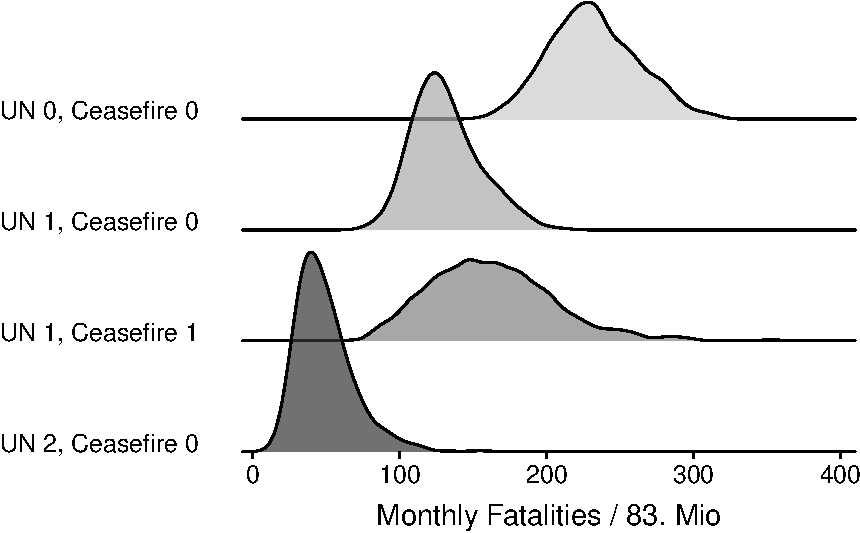
\includegraphics[width=\textwidth]{figs/scenarios-1} \caption[Expected monthly fatalities / 82 Mio]{Expected monthly fatalities / 82 Mio. inhabitants}\label{fig:scenarios}
\vspace{0.5cm} \footnotesize{\textit{Notes: }UN 1 and 2 corresponds to mean and 90th percentile values of UN forces if deployed} \end{figure}

\hypertarget{first-differences}{%
\subsection{First Differences}\label{first-differences}}

For a conclusion of H1 and H2, I simulate the expected effect of UN forces with ceasefire equals 0 and equals 1. Depicting the whole range allows us to observe potential non-linearity in the relationship between our main explaining variables regarding their impact on fatalities. To emphasize the difference between both scenarios, I also compute the first difference between both. Figure \ref{fig:plot-fd} shows the results. The light gray line depicts the expected fatality rate with a ceasefire, the dark gray line without a ceasefire, and the red line represents the first difference. We make the following observations: First, the direction of the impact of ceasefire changes between operations with only a few and operations with many UN forces. This finding corresponds to H2, i.e.~a large number of UN forces is more effective if there is a ceasefire. Second, the uncertainty does also decrease with the stronger UN forces. The reason is that the number of conflicts decreases with the number of forces. Therefore, many of the observations tend to be from the same conflict and thus very similar. We can regard this as a drawback of my approach.

\begin{figure}
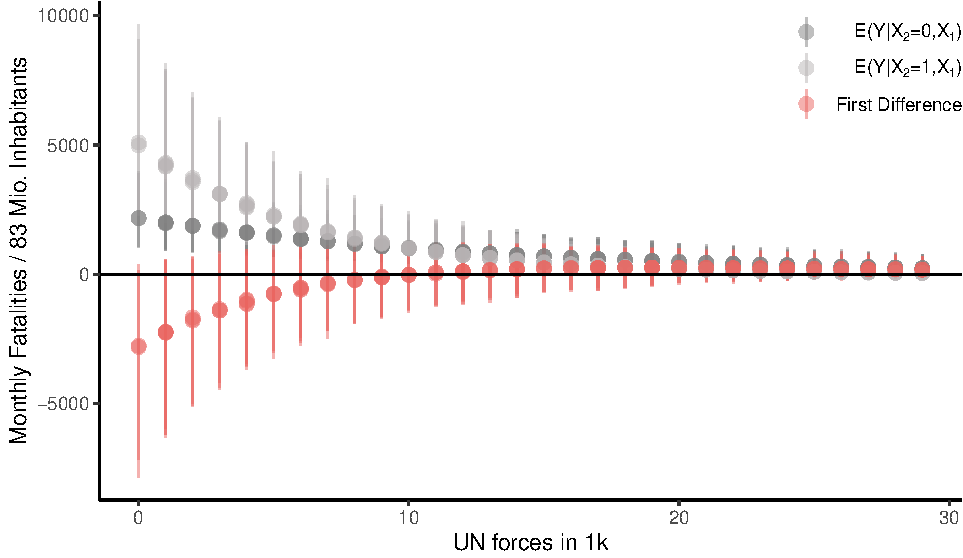
\includegraphics[width=\textwidth]{figs/plot-fd-1} \caption[The effect of ceasefire over the whole range of UN troops]{The effect of ceasefire over the whole range of UN troops}\label{fig:plot-fd}
\vspace{0.5cm} \footnotesize{\textit{Notes: }$X_1$ and $X_2$ correspond to UN Forces and Ceasefire, respectively. First Difference is $E(Y|X_2=1,X_1) - E(Y|X_2=0,X_1)$.} \end{figure}

\hypertarget{robustness-checks}{%
\section{Robustness Checks}\label{robustness-checks}}

To assess the robustness of my findings towards outliers, I recompute model (3) from the set of observations with standardized deviance residuals greater than 2. Both specifications are relatively close. I also test two alternative variants of the main explaining variable UN forces. For this purpose, I decompose UN forces into police and military officers. Then, I recompute model (3) twice again with one of these variables as a substitute for the total number of forces. Again, the coefficients do not change much, although military units appear more effective without a ceasefire, whereas police forces have a higher interaction coefficient.

\hypertarget{conclusion}{%
\section{Conclusion}\label{conclusion}}

In this essay, I analyze two hypotheses. First, whether an increased number of UN troops tends to decrease fatalities of inner-state conflicts. And second, whether this effect tends to be more pronounced when conflict parties are willed to settle the conflict. I found convincing evidence for both hypotheses using a negative binomial model that includes an interaction term and a set of potential confounders. However, this study has the following limitations. First, the number of variables is relatively small. Second, the model assumption that \(Y_1, \dots , Y_n\) are independent appears too strong for panel data. These issues can be addressed by future research.
\newpage

\hypertarget{references}{%
\section*{References}\label{references}}
\addcontentsline{toc}{section}{References}

\singlespacing

\hypertarget{refs}{}
\begin{CSLReferences}{1}{0}
\leavevmode\vadjust pre{\hypertarget{ref-agresti2015foundations}{}}%
Agresti, Alan. 2015. \emph{Foundations of Linear and Generalized Linear Models}. John Wiley \& Sons.

\end{CSLReferences}

\clearpage

\hypertarget{statutory-declaration}{%
\section*{Statutory Declaration}\label{statutory-declaration}}
\addcontentsline{toc}{section}{Statutory Declaration}

Hiermit versichere ich, dass diese Arbeit von mir persönlich verfasst ist und dass ich keinerlei fremde Hilfe in Anspruch genommen habe.
Ebenso versichere ich, dass diese Arbeit oder Teile daraus weder von mir selbst noch von anderen als Leistungsnachweise andernorts eingereicht wurden.
Wörtliche oder sinngemäße Übernahmen aus anderen Schriften und Veröffentlichungen in gedruckter oder elektronischer Form sind gekennzeichnet.
Sämtliche Sekundärliteratur und sonstige Quellen sind nachgewiesen und in der Bibliographie aufgeführt.
Das Gleiche gilt für graphische Darstellungen und Bilder sowie für alle Internet-Quellen.
Ich bin ferner damit einverstanden, dass meine Arbeit zum Zwecke eines Plagiatsabgleichs in elektronischer Form anonymisiert versendet und gespeichert werden kann.
Mir ist bekannt, dass von der Korrektur der Arbeit abgesehen werden kann, wenn die Erklärung nicht erteilt wird.

\SignatureAndDate{}
\renewcommand*{\thepage}{ }

\noindent I hereby declare that the paper presented is my own work and that I have not called upon the help of a third party.
In addition, I affirm that neither I nor anybody else has submitted this paper or parts of it to obtain credits elsewhere before.
I have clearly marked and acknowledged all quotations or references that have been taken from the works of other.
All secondary literature and other sources are marked and listed in the bibliography.
The same applies to all charts, diagrams and illustrations as well as to all Internet sources.
Moreover, I consent to my paper being electronically stores and sent anonymously in order to be checked for plagiarism.
I am aware that the paper cannot be evaluated and may be graded \enquote{failed} (\enquote{nicht ausreichend}) if the declaration is not made.

\SignatureAndDateEng{}

% % % 
\end{document}
